\documentclass[10pt,letterpaper]{article}

\usepackage[pdftex]{graphicx}

\begin{document}
	
	\section{Quadric Surfaces}
	
	\subsection{Elliptic Cylinder}
	\[  \frac{x^2}{a^2}+\frac{y^2}{b^2} = 1 \]
	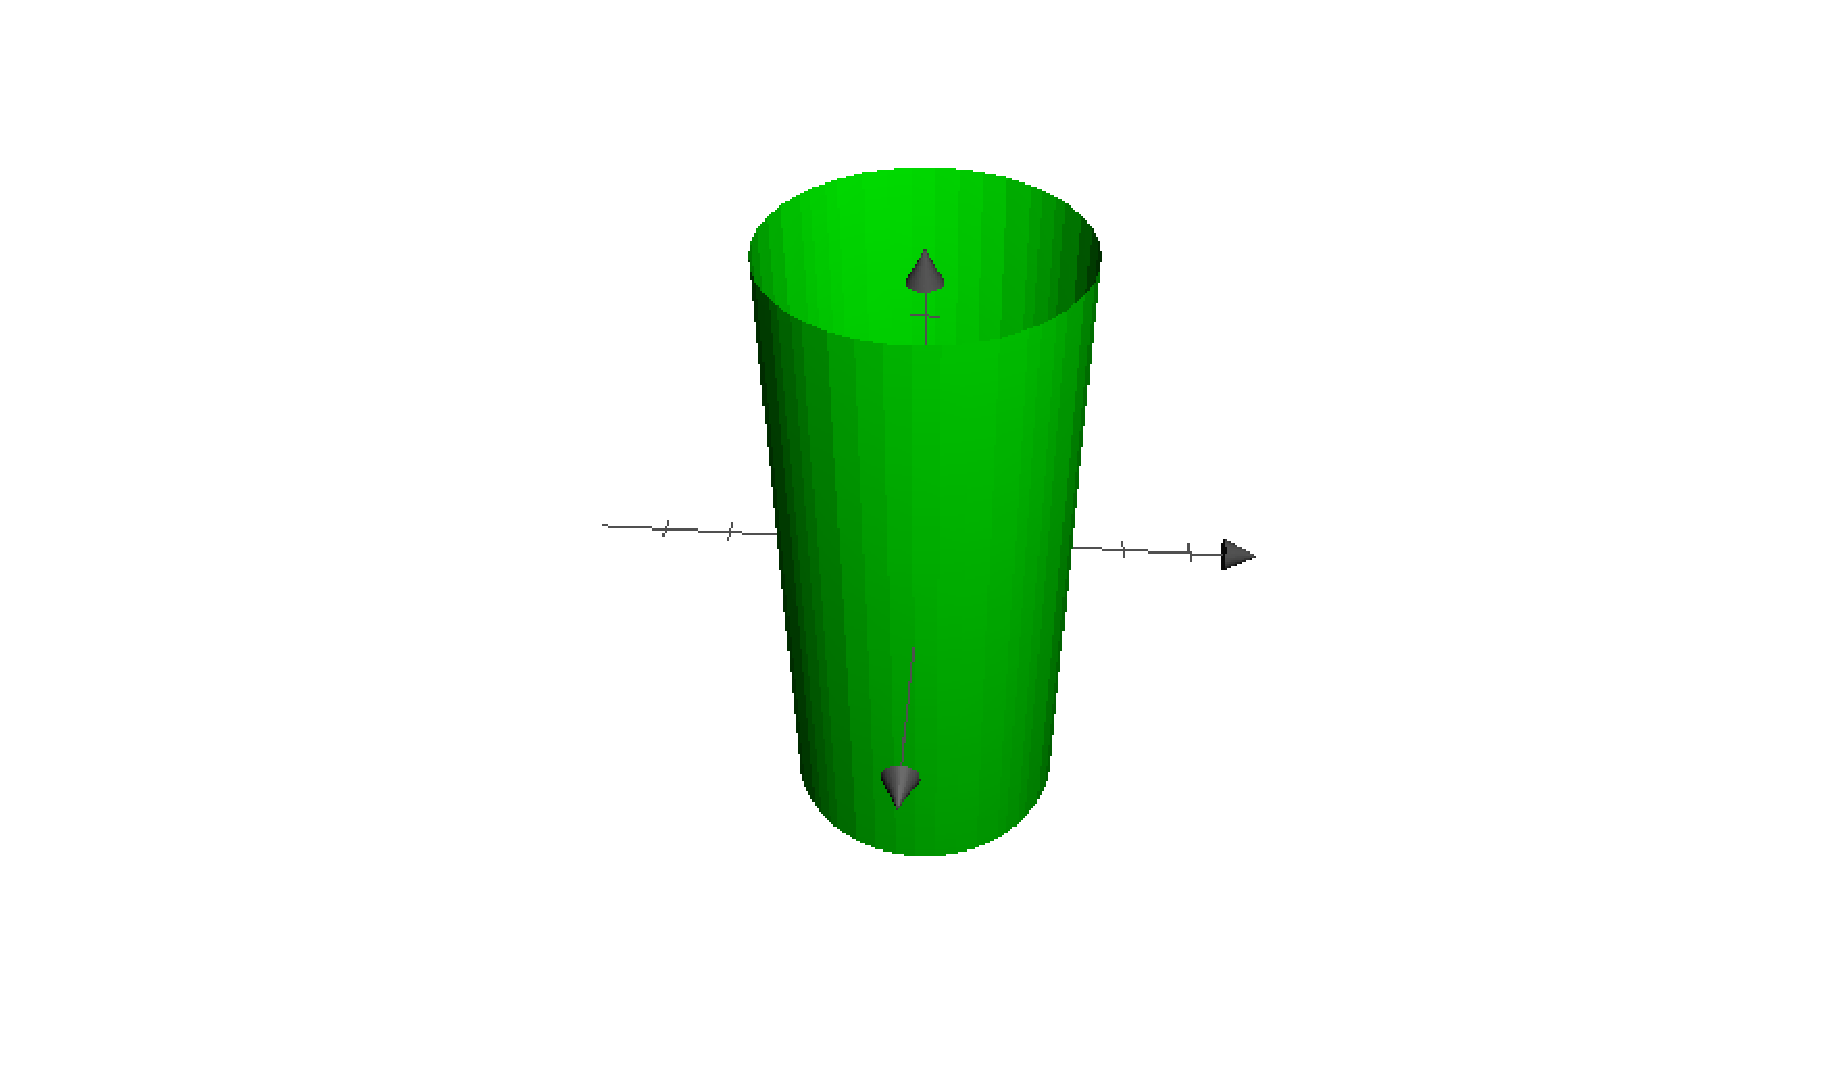
\includegraphics[width=4.5in]{ellipticcylinder.pdf}

	\subsection{Hyperbolic Cylinder}
	\[  \frac{x^2}{a^2}-\frac{y^2}{b^2}=1 \]
	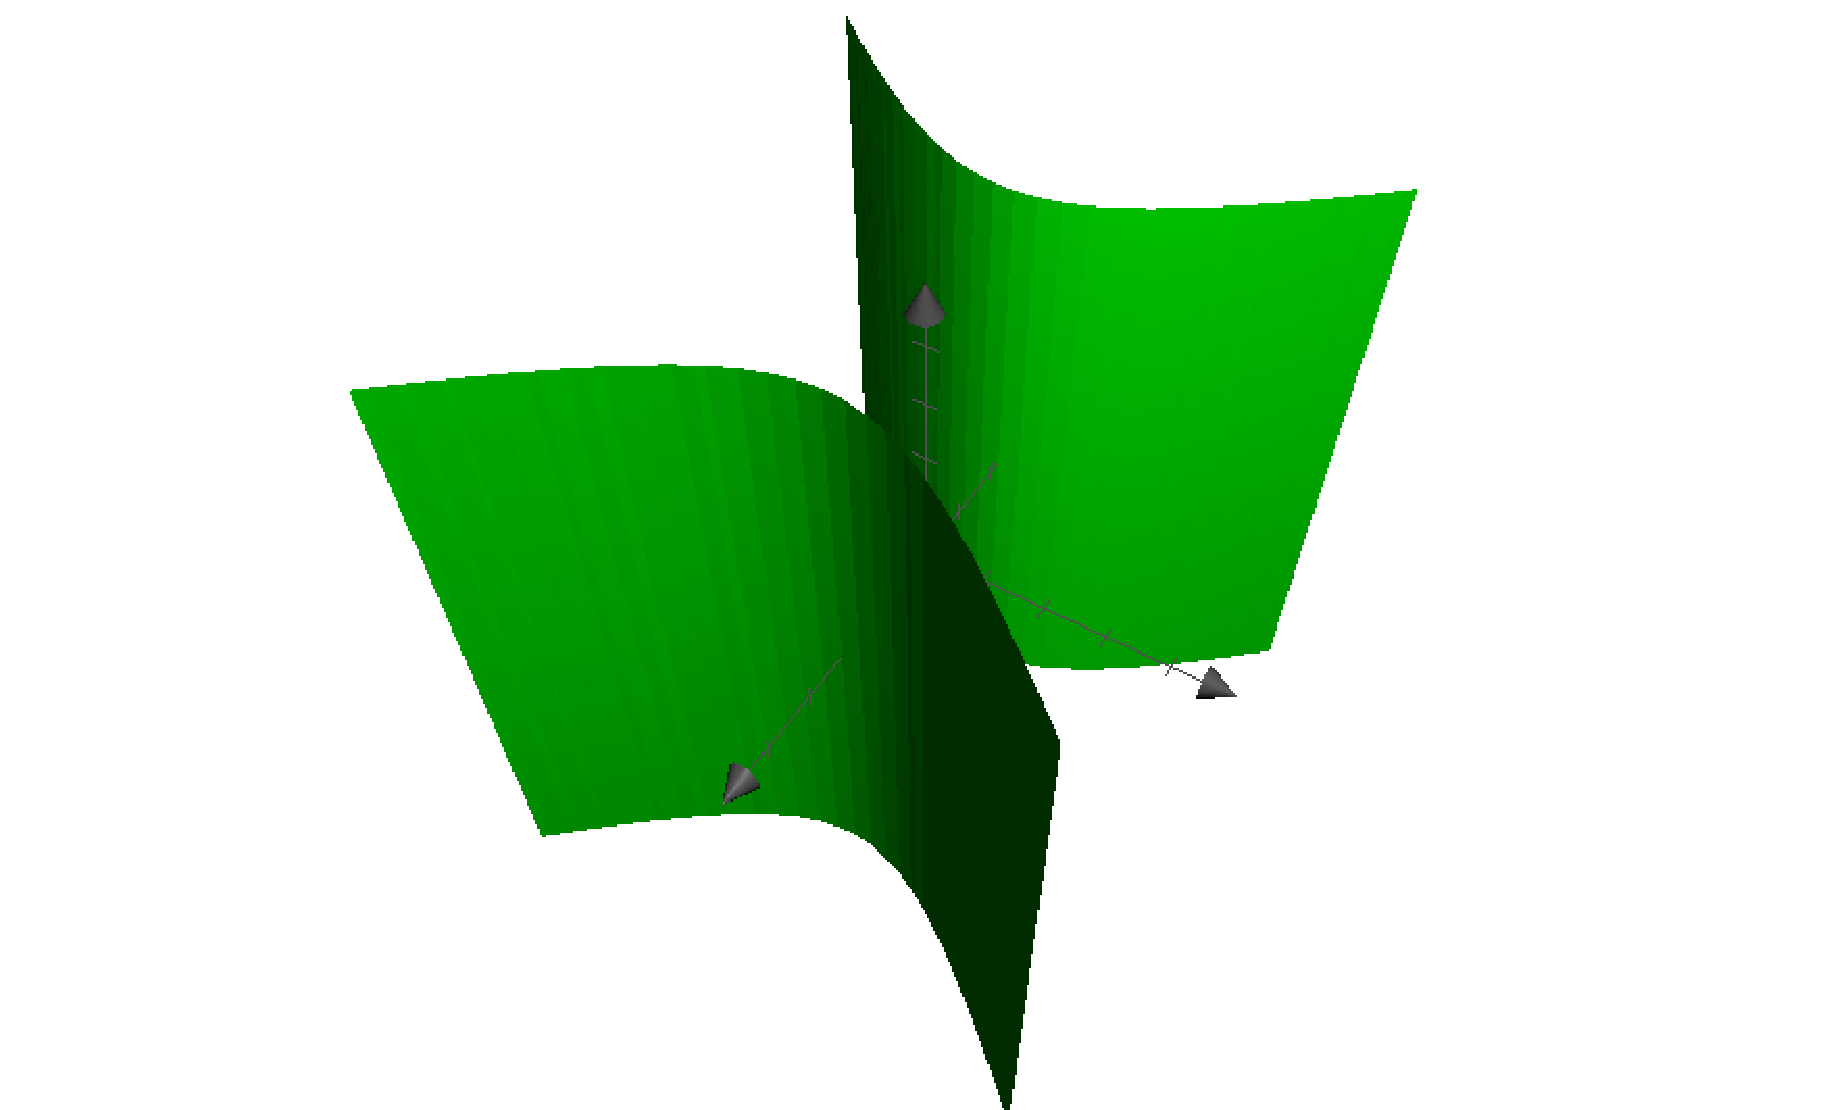
\includegraphics[width=4.5in]{hyperboliccylinder.pdf}
	\newpage

	\subsection{Parabolic Cylinder}
	\[  z=Ax^2 \]
	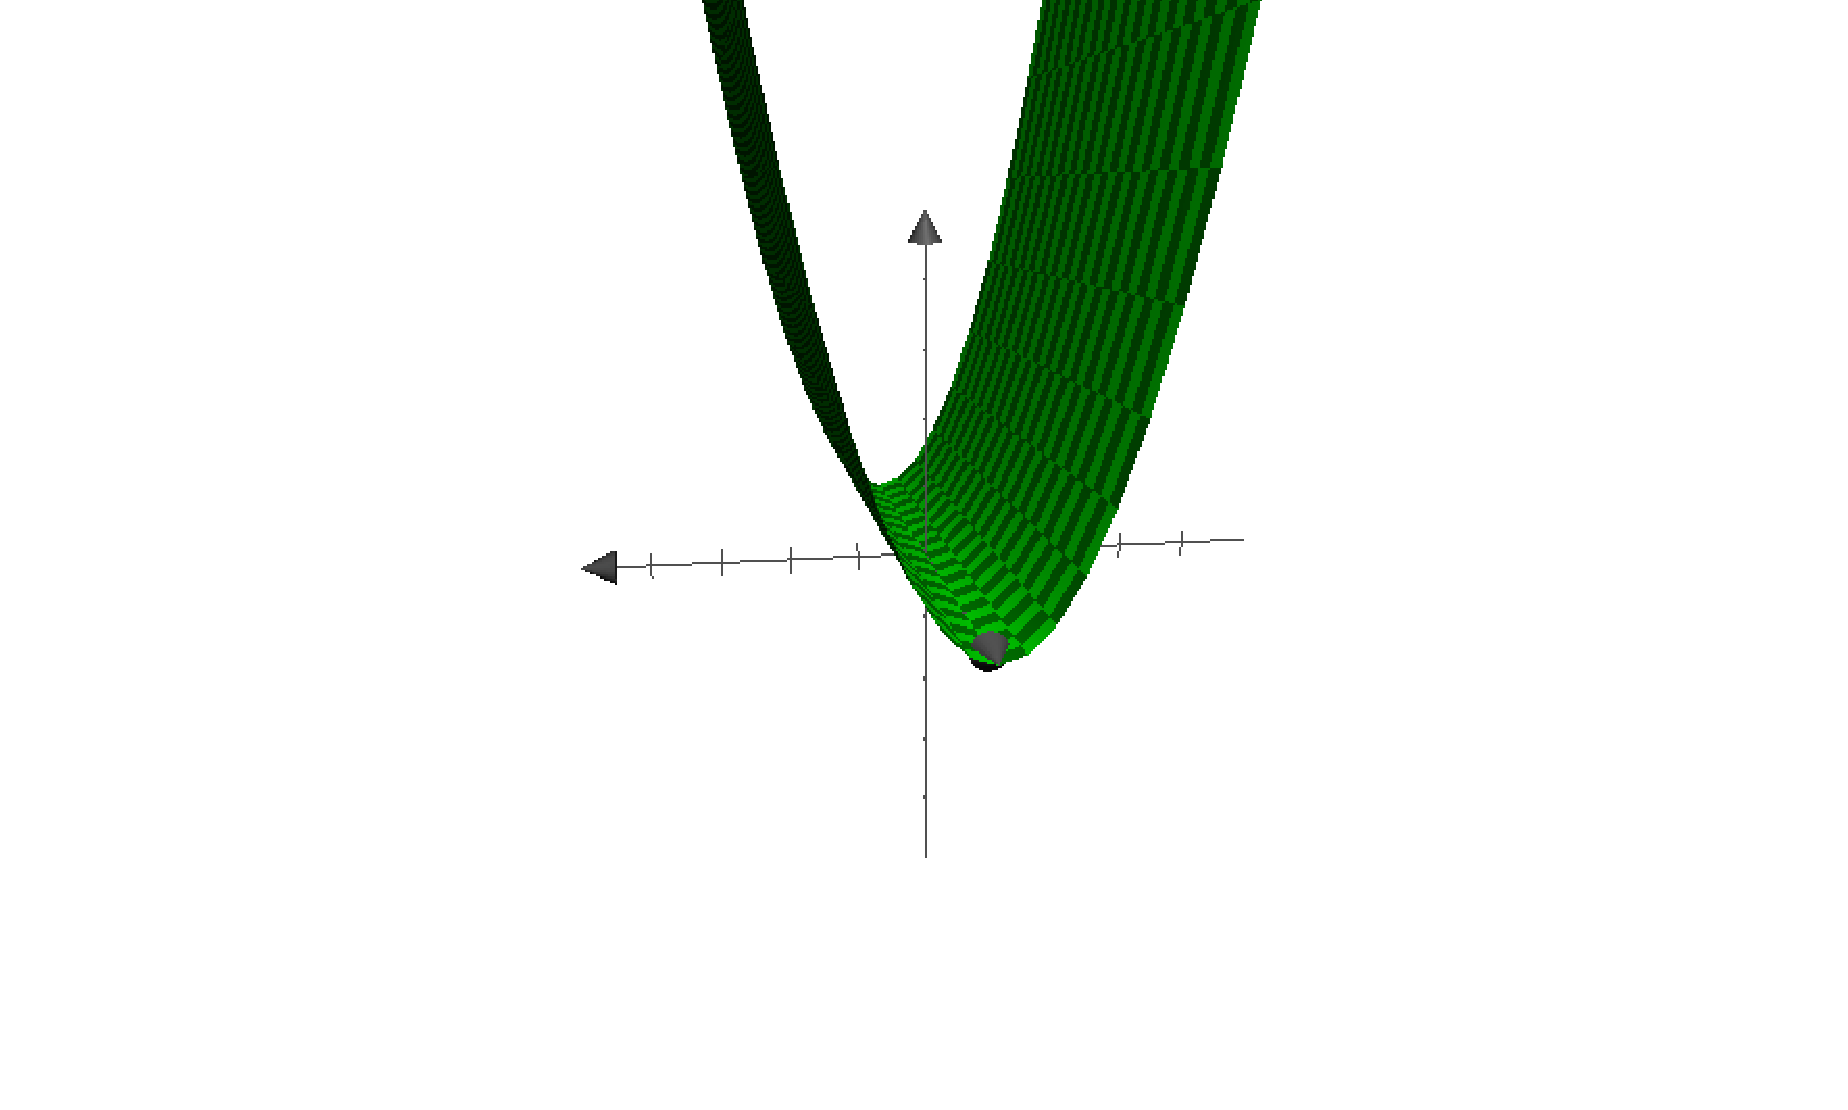
\includegraphics[width=4.5in]{paraboliccylinder.pdf}
	
	\subsection{Ellipsoid}
	\[ \frac{x^2}{a^2}+\frac{y^2}{b^2}+\frac{z^2}{c^2} =1 \]
	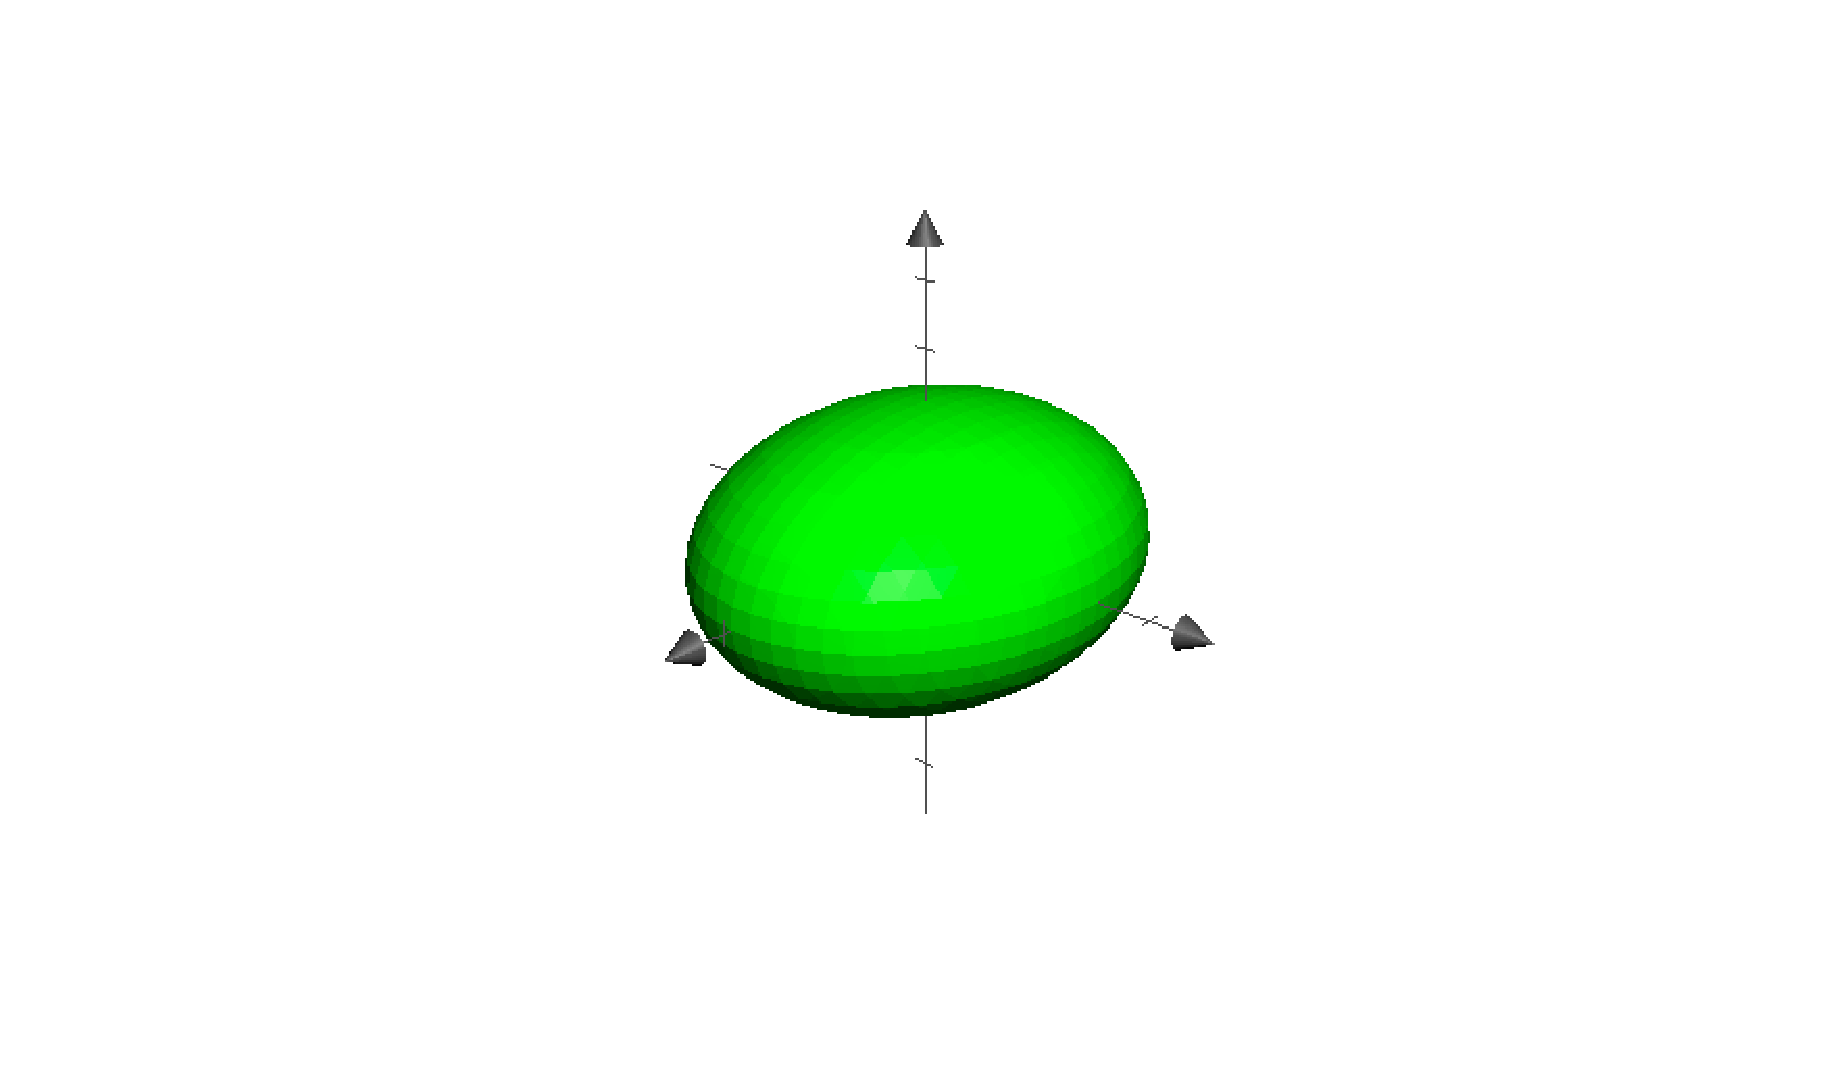
\includegraphics[width=4.5in]{ellipsoid.pdf}
	\newpage
	
	\subsection{Parabaloid}
	\[  z = \frac{x^2}{a^2}+\frac{y^2}{b^2} 	\]
	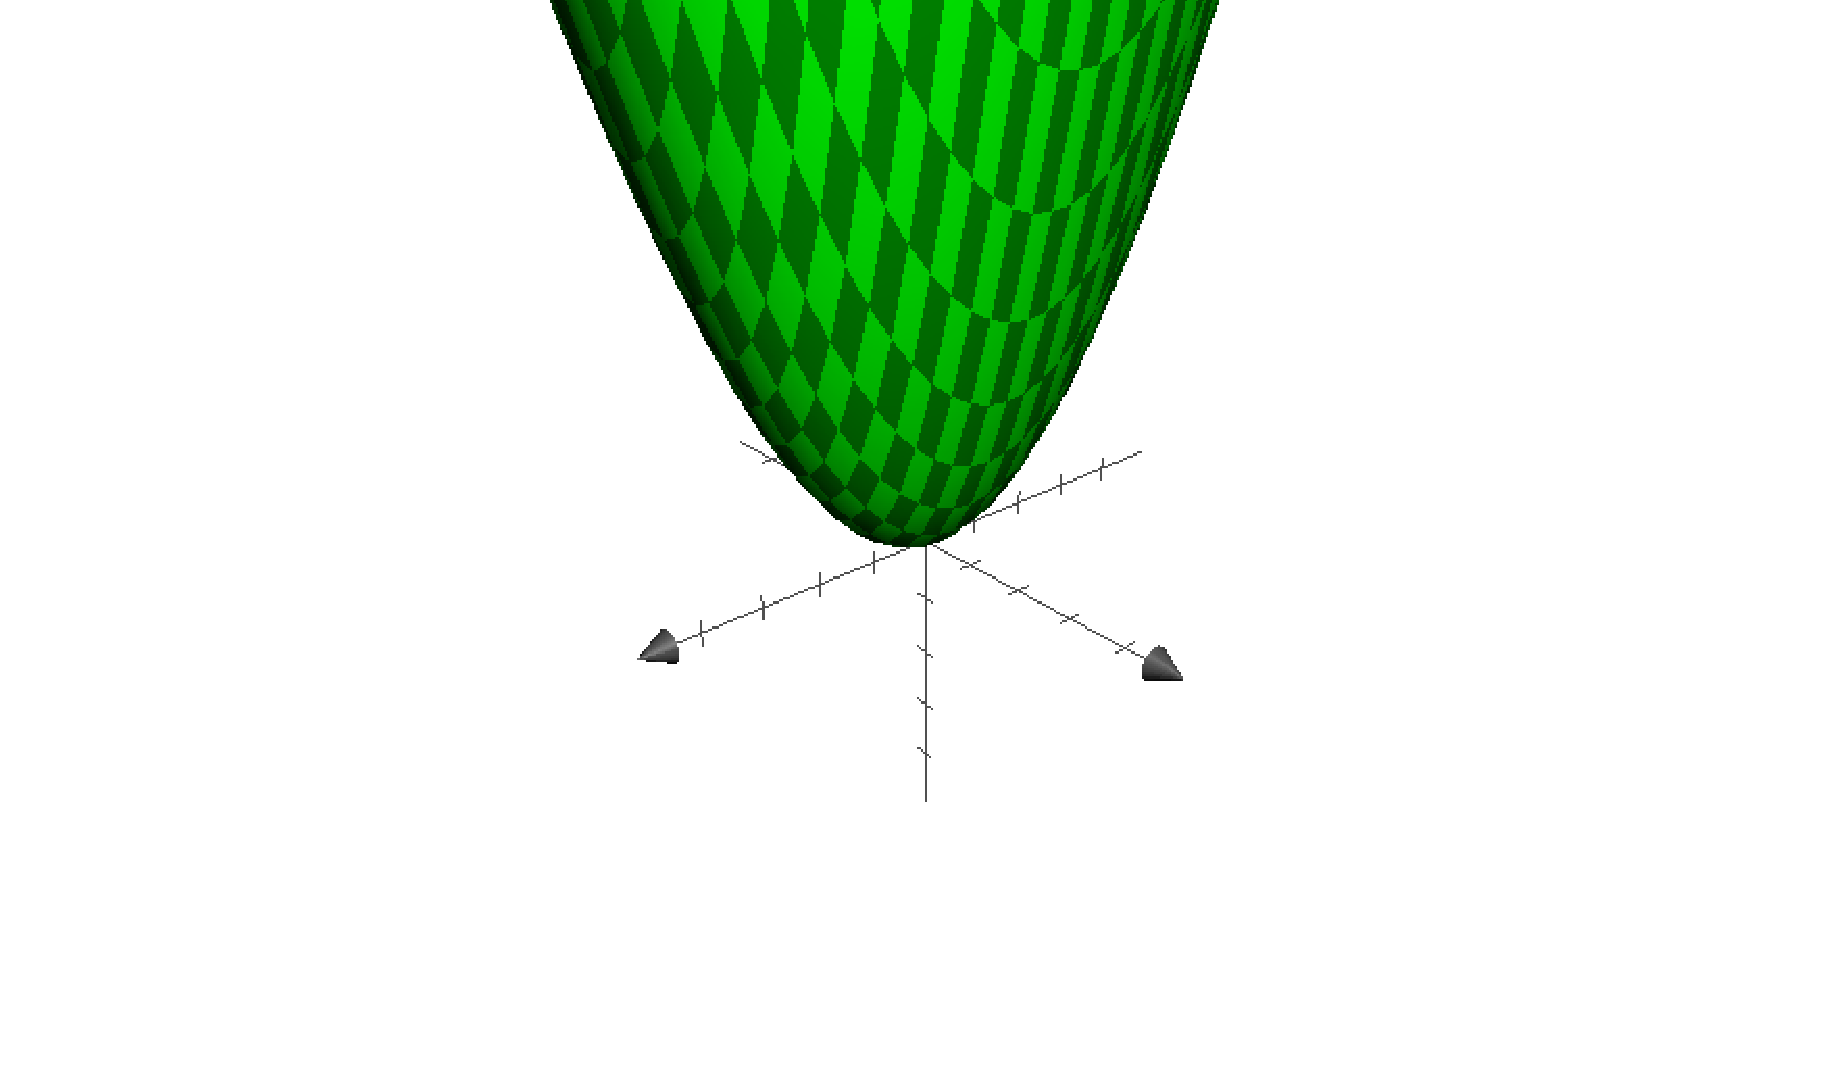
\includegraphics[width=4.5in]{paraboloid.pdf}
		
	\subsection{Elliptic Cone}
	\[  z^2 = \frac{x^2}{a^2}+\frac{y^2}{b^2}	\]
	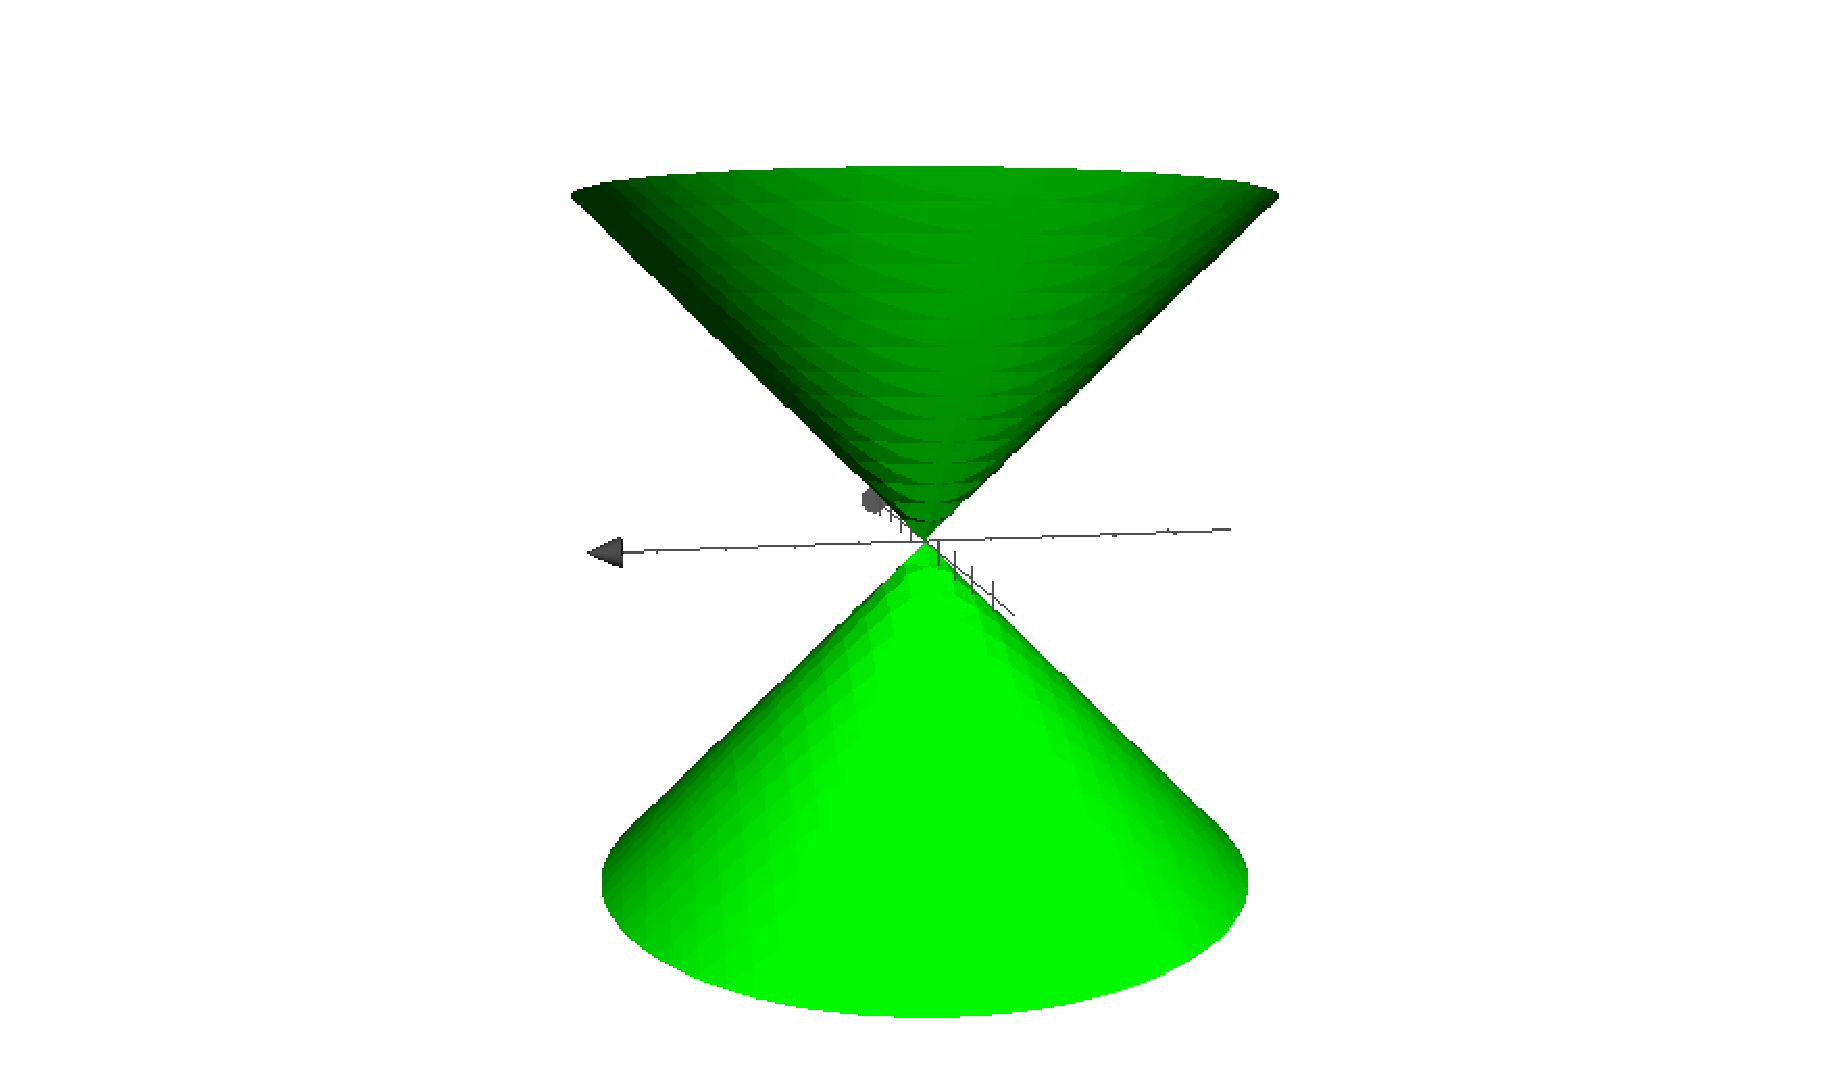
\includegraphics[width=4.5in]{ellipticcone.pdf}
	\newpage
	
	\subsection{Hyperbolic Paraboloid}
	\[ z=\frac{x^2}{a^2}-\frac{y^2}{b^2}  \]
	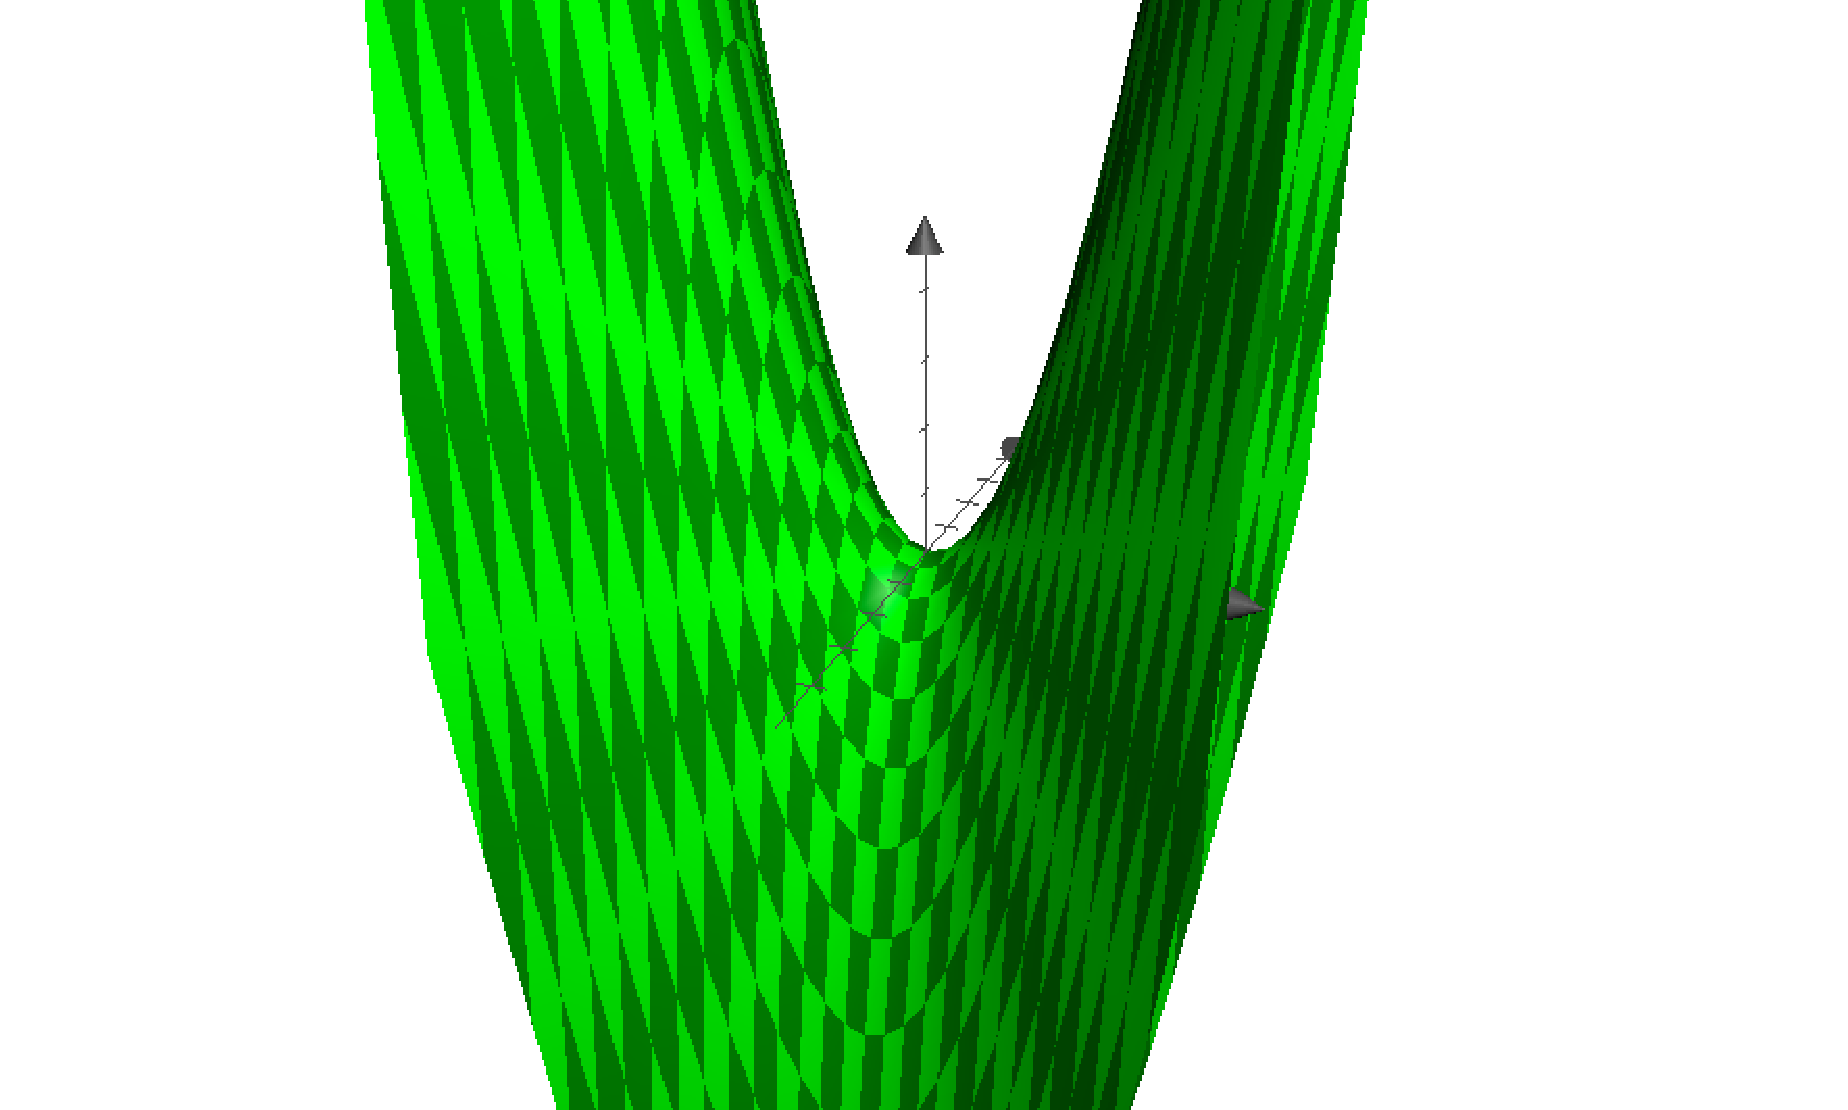
\includegraphics[width=4.5in]{hyperbolicparoboloid.pdf}
		
	\subsection{Elliptic Paraboloid of One Sheet}
	\[  \frac{x^2}{a^2}+\frac{y^2}{b^2}-\frac{z^2}{c^2}=1 \]
	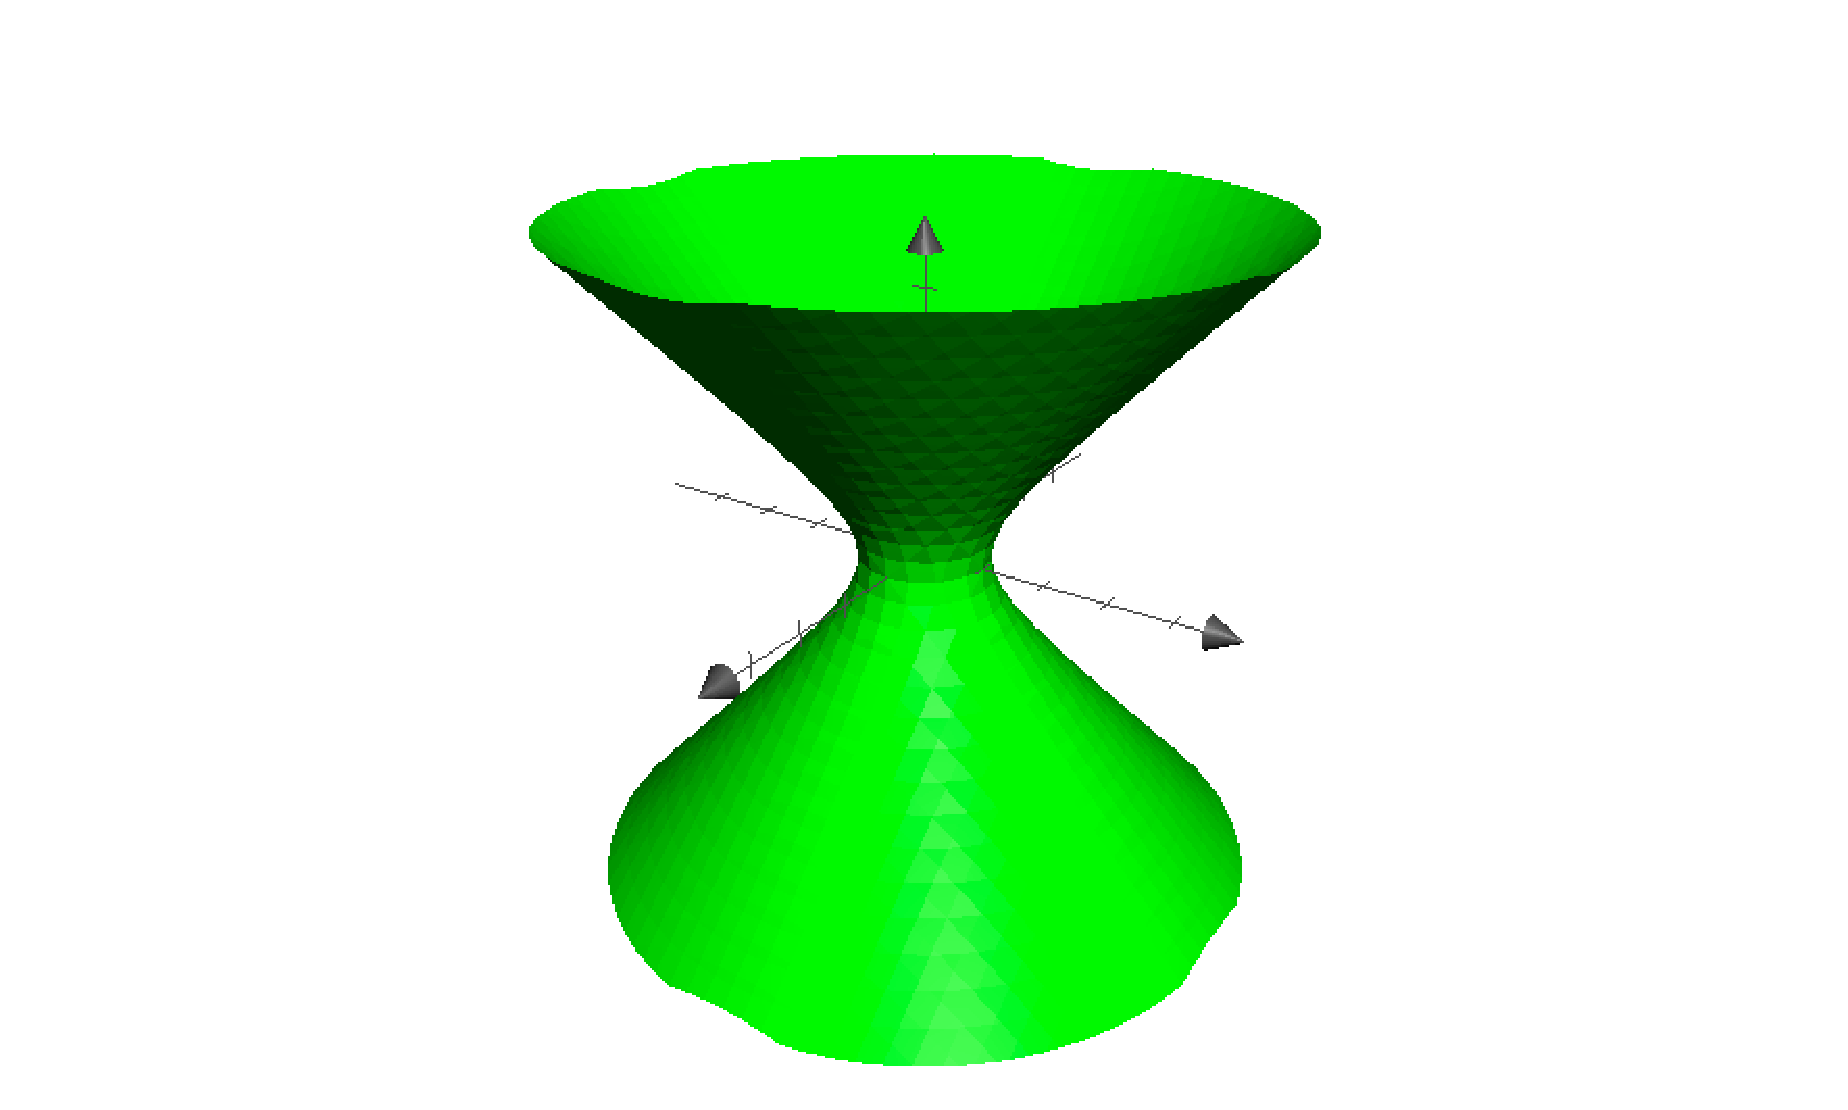
\includegraphics[width=4.5in]{elliptichyperboloid1.pdf}
	\newpage
		
	\subsection{Elliptic Paraboloid of Two Sheets}
	\[  -\frac{x^2}{a^2}-\frac{y^2}{b^2}+\frac{z^2}{c^2}=1 \]
	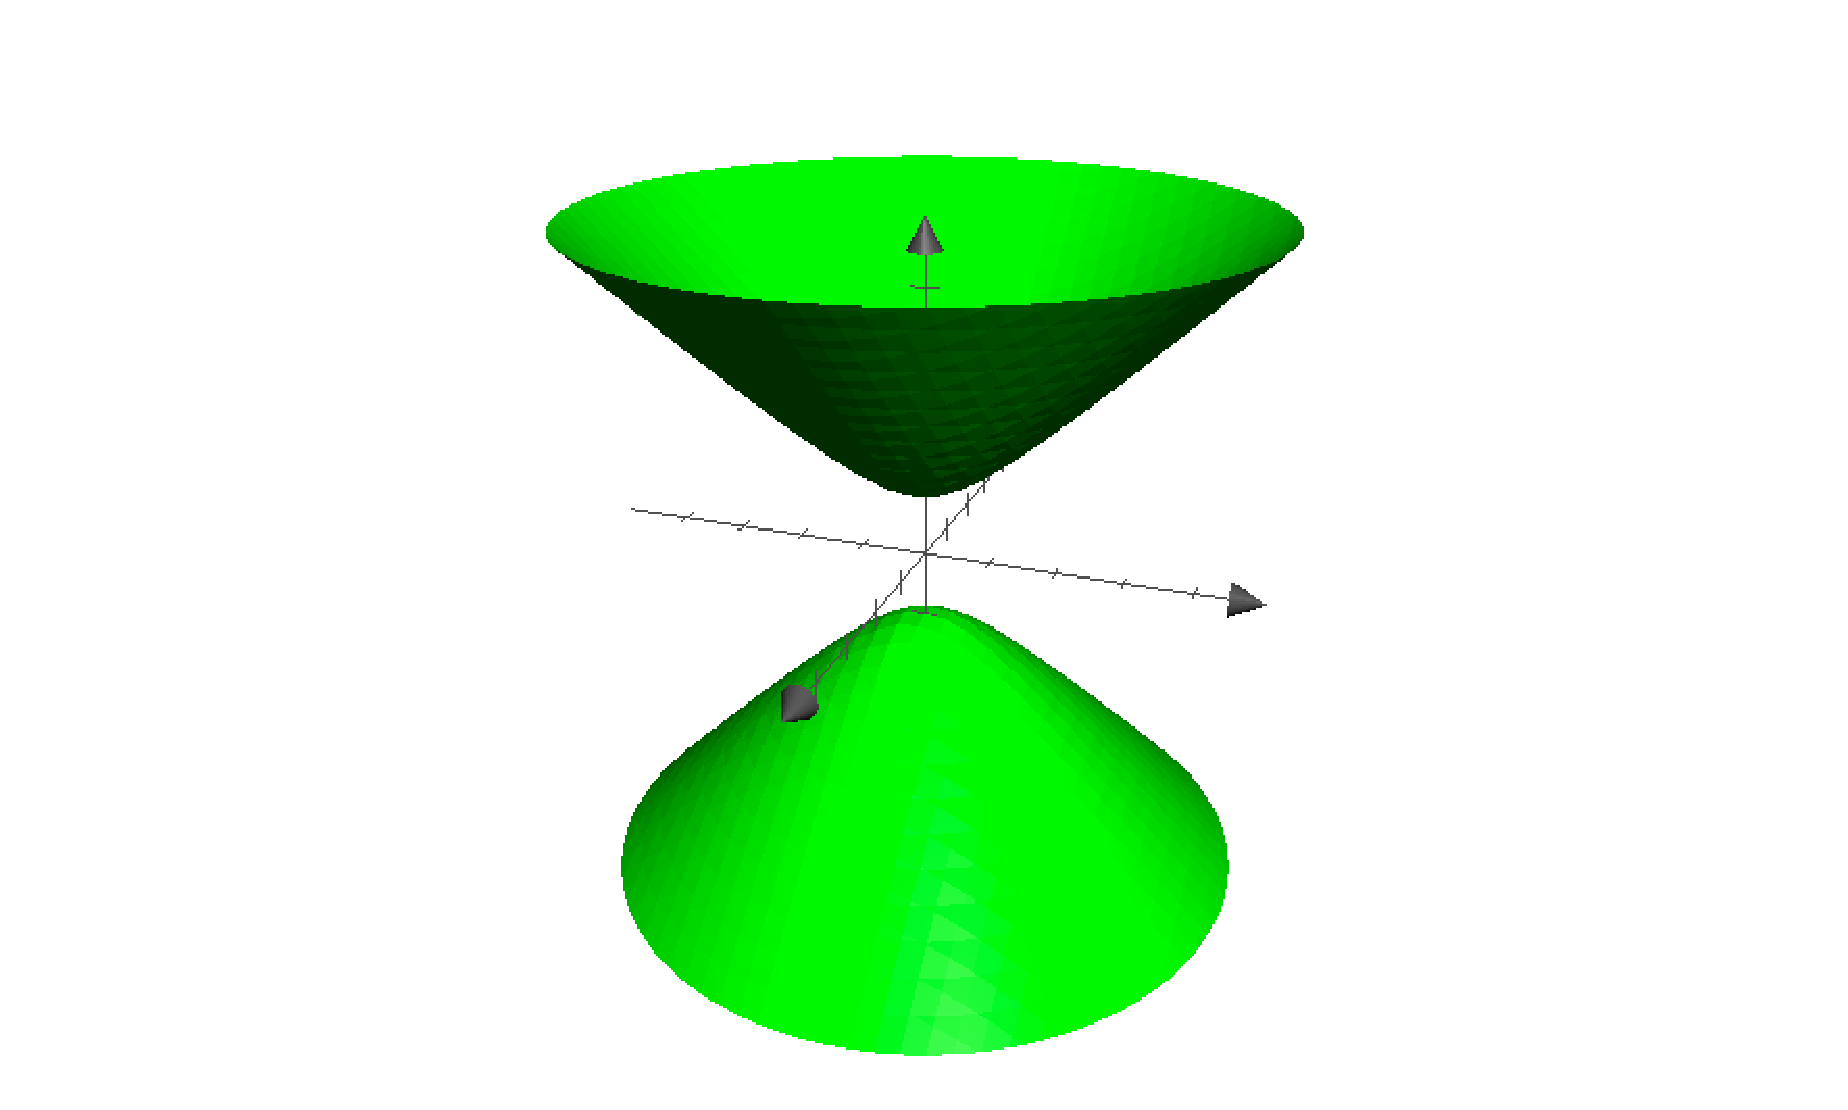
\includegraphics[width=4.5in]{elliptichyperboloid2.pdf}
	
\end{document}